\section{Requirements-Engeneering}
Das \textbf{Lastenheft} beschreibt die gesamte Funktionalität, die eine Software erfüllen soll, und dient als Grundlage für die Einholung von Angeboten und wird aus sicht des Auftraggebers geschrieben. Das \textbf{Pflichtenheft} stellt die Softwarelösung des Anbieters dar und beschreibt, wie die im Lastenheft gewünschten Funktionen umgesetzt werden.

\subsection{Stackholder}
Stackholder sind Persona, welche mit dem System interagieren. Dies können einzelene Personen oder auch Gruppen bzw. andere Sofware-Teile sein. Sie müssen sehr sorgfälltig evaluiert werden, um nachfolgend die Anforderungen sauber zu definieren.

\subsection{Kontextabgrenzung}
Stellt sicher, das ein System von der Umwelt abgeschottet ist. Oft wird zur Übersicht ein Diagram erstellt, welche die Grenzen klar darstellt. Folgendes Beispiel für einen SPICE Simulator, welcher drei Sub-Systeme beinhaltet. Jedes dieser Sub-System kommuniziert über einen definierten Kanal.
\begin{center}
	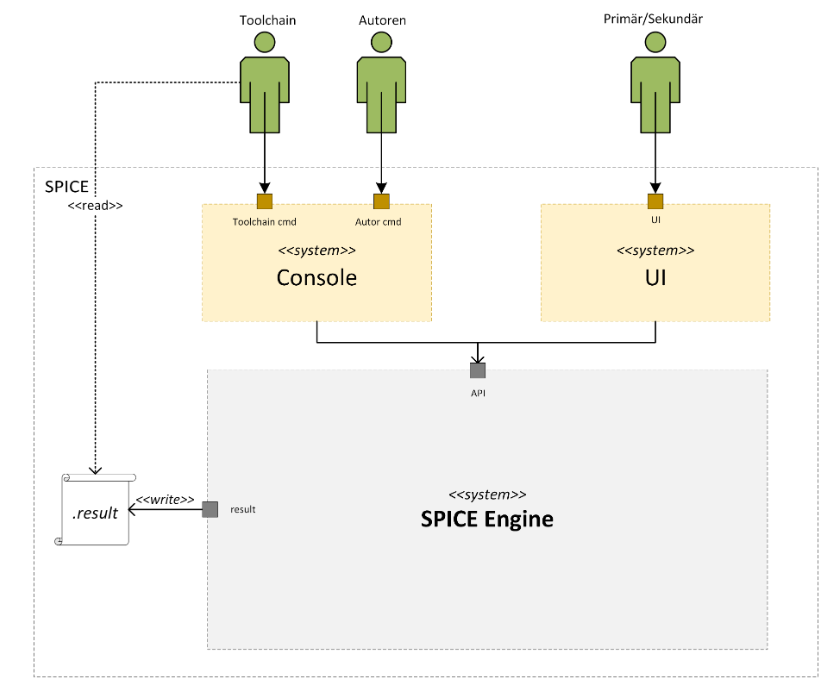
\includegraphics[width=\columnwidth]{Images/kontextabgrezung}
\end{center}

\subsection{Anforderungen}
Anforderungen werden häufig in folgende Gruppen unterteilt: 
\begin{itemize}[nosep]
	\item Funktionale Anforderungen
	\item Nichtfunktionale Anforderungen
	\item Rahmenbedingungen
\end{itemize}

\subsubsection{Nichtfunktionale Anforderungen} sind jene, welche gefodert werden, aber keine neuen Funktionen beiten. zB Qualitätsanforderungen (Genauigkeit, Verfügbarkeit, Zuverlässigkeit). Diese Anforderungen betreffen meist mehrere Funktionalen Anforderungen und können sich auch gegenseitig beeinflussen (Sicherheit vs Benutzerfreundlichkeit)

\subsubsection{Funktionale Anforderungen} lassen sich gut mittels Use-Case Diagram beschreiebn. Sie definieren welche Eigeschaften ein System hat und welche Funktionalität erwartet werden kann. zB Tempo Messen
\begin{center}
	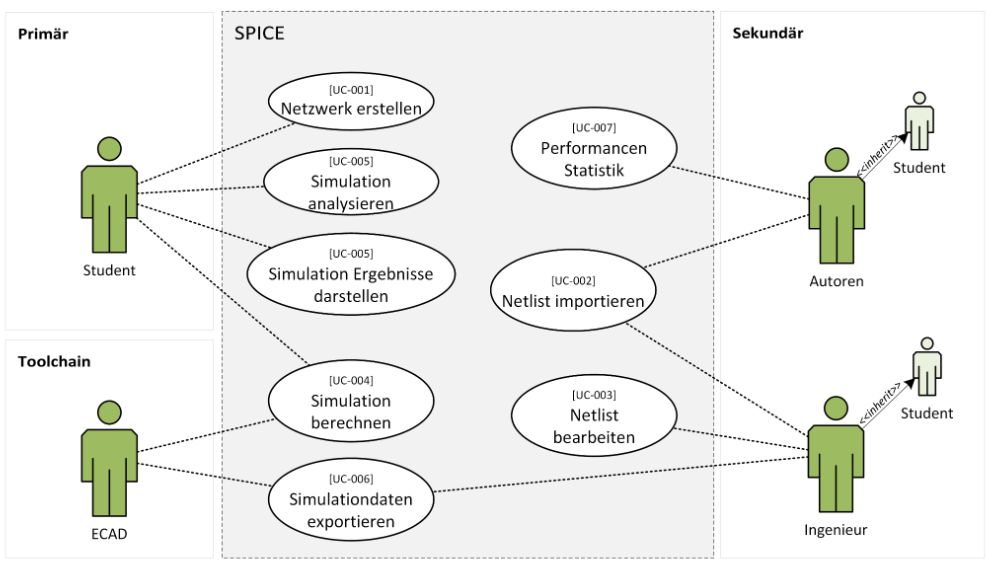
\includegraphics[width=\columnwidth]{Images/usecase}
\end{center}


\subsubsection{Rahmenbedingungen} sind im gegensatz zu Anforderungen Einschränkungen. \underline{Technische} Rahmenbedingungen sind zB \textit{Software muss auch Windows lauffähig sein}, \textit{Git muss eingesetzt werden}. etc. Des weiteren sind \underline{organisatorische} Rahmenbedingungen zB \textit{Team ist 4 Mann gross}. Rahmenbedingungen können grundsätzlich nicht geändert werden und vordern oft vordefinierte Lösungen (Was gute Anforderungen auf keinen Fall tun sollten).

\subsubsection{Vorgehen}
Das vorgehen, um gute Anforderungen zu definieren ist schwierig. Oft werden Stakeholder mittels Interview befragt oder Selbstaufschreibung.  
\begin{center}
	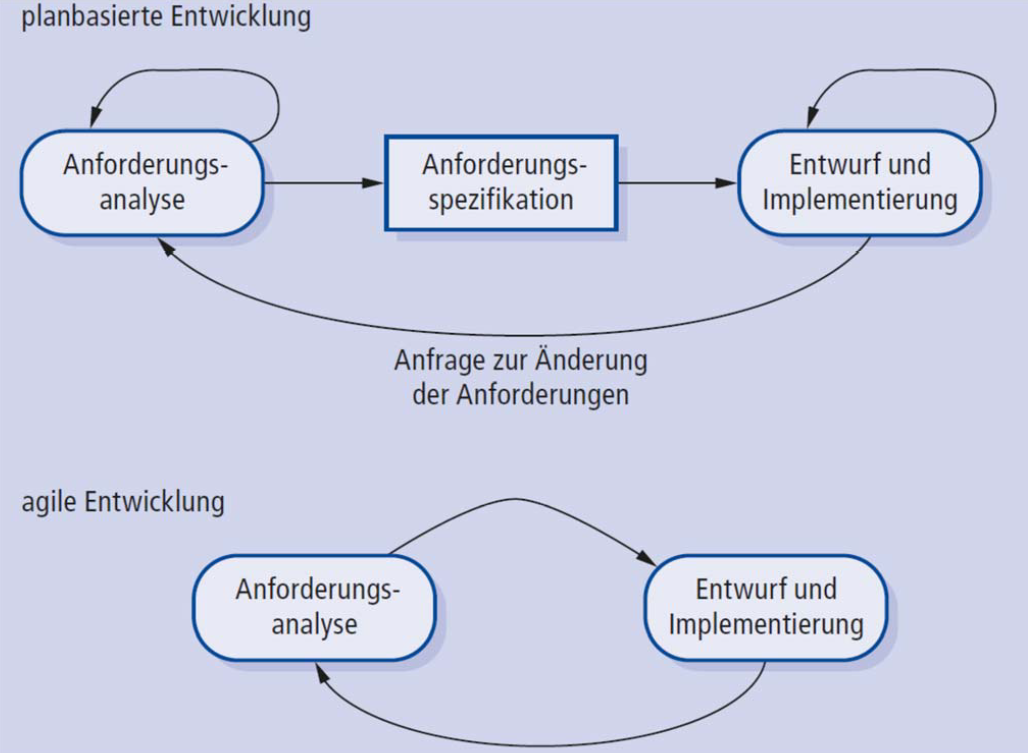
\includegraphics[width=0.8\columnwidth]{Images/requirements_engeneering}
\end{center}

~\\
\textbf{Tips} für Anforderung: Anforderungen müssen überprüfbar, eindeutig, vollständig, realisierbar und gültig sein.
\begin{center}
	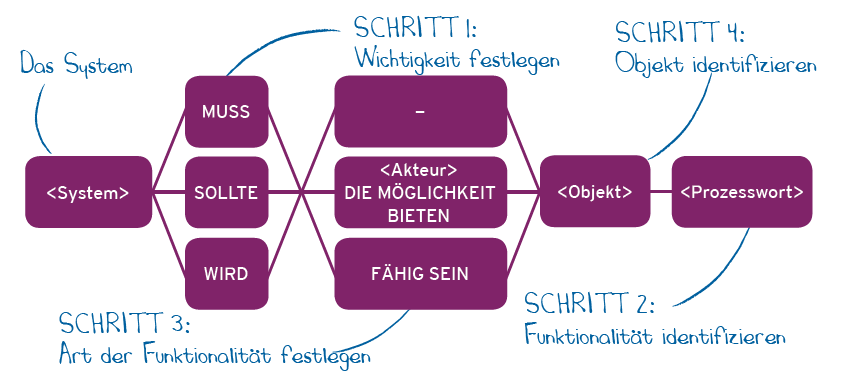
\includegraphics[width=\columnwidth]{Images/schablone}
\end{center}

